\documentclass[]{article}
\usepackage[round]{natbib}

\usepackage{fullpage}
\usepackage{listings}
\usepackage{url}
\usepackage{authblk}
\usepackage{graphicx}
\usepackage{color}
\usepackage{booktabs}
\usepackage{amsfonts}

\lstset{language=Python}

% cross-reference with main text
\usepackage{xr}
\externaldocument{paper}

% local definitions
\newcommand{\sgcomment}[1]{{\textcolor{red}{SG: #1}}}
\newcommand{\bmhcomment}[1]{{\textcolor{blue}{BMH: #1}}}
\newcommand{\aprcomment}[1]{{\textcolor{magenta}{APR: #1}}}
\newcommand{\tdwcomment}[1]{{\textcolor{cyan}{TDW: #1}}}

\newcommand{\E}{\mathbb{E}}

\usepackage{array}
\newcolumntype{P}[1]{>{\raggedright\arraybackslash}p{#1}}

\begin{document}
\title{Supporting Information for\\
``A weakly structured stem for human origins in Africa''}
\author{Aaron P. Ragsdale, Timothy D. Weaver, Brenna M. Henn, and Simon Gravel}
\date{\today}
\maketitle

\renewcommand{\thefigure}{S\arabic{figure}}
\renewcommand{\thetable}{S\arabic{table}}
\renewcommand{\theequation}{S\arabic{equation}}
\setcounter{figure}{0}
\setcounter{table}{0}
\setcounter{equation}{0}

\tableofcontents
\newpage

\section{Data and sequencing}

\subsection{Sequencing and variant calling}

Low coverage (4-8x) Illumina short read data were generated for the Nama,
Gumuz, Amhara and Oromo populations as part of the African Diversity Reference
Panel (Sanger / Wellcome Trust) \citep{Gurdasani2015-qy,Pagani2015-pz} and
approved through a secondary data analysis agreement for this project. Briefly,
raw reads were aligned to GRCH37 with BWAmem \aprcomment{cite}, duplicates
marked with Picard MarkDuplicates, reads were realigned around indels with GATK
RealignerTargetCreater / IndelRealigner followed by BQSR with dbSNP 137.
Contamination checks were performed requiring that FREEMIX $<0.05$;
contamination checks resulted in the elimination of 22 Nama samples. We note
that the high heterozygosity in these genomes both due to inherent genetic
diversity and admixture may have violated base assumptions for this
heterozygosity check. Genomes were then variant called with GATK3.2 Unified
Genotyper \aprcomment{cite} using joint calling across 2,478 individuals within
the ADRP dataset with a minimum base quality of 17. Data were merged with 1000
Genomes Phase 3 \citep{1000_Genomes_Project_Consortium2015-zq} using the union
of sites identified with bcftools isec (-n+1) \aprcomment{cite} then refined
with Variant Recalibrator with a truth sensitivity threshold of 99.5\%. HapMap
III and dbSNP 138 served as known sites while 1000 Genomes Phase 1 Omni2.5 and
Phase 1 genomic SNP served as the training set. After VR, no batch effects were
observed along PC1 and PC2 for 1000 Genomes vs. ADRP. Phasing on the combined
dataset was performed via SHAPEIT2 \aprcomment{cite} and utilized the duoHMM
option for duos and trios. We highlight 82 Nama genomes which are newly
available (unpublished) under accession number EGAD00001006198. Among these 82
Nama samples, we down-sampled the individuals to minimize close relatives and
admixture, such that 44 Nama genomes were retained. 2nd and 3rd degrees
relatives were inferred from reconstructed pedigrees with Omni2.5 SNP array
data. Individuals with $>70\%$ estimated Khoe-San ancestry were retained for
analysis, after partitioning ancestry into $k=6$ clusters with ADMIXTURE
\aprcomment{cite} where alternative ancestries represent European, West
African, Near Eastern, and East African gene flow. 

\subsection{Nama sample collection and consent}

DNA samples were collected from three Nama communities in the Richtersveld
region of South Africa, which borders southern Namibia, in 2012. A community
guide was present during each interview and facilitated consent in Afrikaans or
Nama. Written consent was recorded per our IRB protocol with human subjects
approval from Stanford University (Protocol \#13829), Stellenbosch University
(N11/07/210) and later maintained via SUNY Stony Brook (Protocol \#727494).
Saliva samples were extracted from Oragene [OGR-500] kits at Stellenbosch
University. Results stemming from genetic analyses have been communicated in
2015, 2019, 2021 via community presentations, a radio interview and to
representatives of the Richtersveld National Park.

\subsection{Details about populations used in analyses}

\sgcomment{To be expanded. TODO: Brenna}
\begin{itemize}
    \item From the merged dataset of the African Diversity Reference Panel and
        1000 Genomes phase 3 data, subsampled to population included in this study
    \item West Africa: Mende from Sierra Leone (MSL); South Africa: newly sequenced 
        Nama; East Africa: Gumuz (traditionally hunter-gatherer with low levels of 
        Eurasian admixture), Oromo and Amhara (combined as traditionally 
        agriculturalists with large proportion of back-to-Africa Eurasian ancestry); 
        Eurasian: British (GBR)
    \item Combined with the high coverage Vindija neanderthal genome
    \item For running Relate, we used a larger set of populations. We kept all 
        African 1000 Genomes populations, along with the Nama, Gumuz, Oromo, and
        Amhara, as well as 4 Eurasian populations from 1000 Genomes: GBR, CEU, PJL,
        and CHB
\end{itemize}

\subsection{Filtering and subsetting data}

All analyses presented in this work focus on biallelic single nucleotide
polymorphisms within the 1000 Genomes Phase 3 strict mask.  For the moments-LD
analysis, we focused on intergenic locations because these appear less affected
by natural selection compared to both synonymous and nonsynonymous variation
\citep{Ragsdale2018-dd}. To enable comparison with Neanderthal DNA, we excluded
regions for which the Vindija Neanderthal sample had less than 100 contiguous
base pairs. 

\section{Computing statistics}

\subsection{LD and diversity statistics used in model fits}

We used multi-population linkage disequilibrium (LD) and pairwise diverisity
statistics to fit demographic models to data. These statistics, introduced and
described in detail in \citet{Ragsdale2019-nt}, are the multi-population analog
of the classic LD statistics first described and computed by
\citet{Hill1968-vu,Ohta1971-yd}.

Given two biallelic loci, with alleles $A$ and $a$ and the left locus and
allels $B$ and $b$ at the right locus, the standard covariance measure of LD is
$D=p_{AB}p_{ab}-p_{Ab}p_{aB}$, where $p_{AB}$ is the frequency of $AB$
haplotypes in a population (and thus the probability of drawing an $AB$
haplotype in a random sample of that population). \citet{Hill1968-vu} solve for
the expectation of $D^2$ using a system of equations that includes
$\E[Dz] = \E[D(1-2p_A)(1-2p_B)]$ and $\E[\pi_2] =
\E[p_A(1-p_A)p_B(1-p_B)]$, where $p_A$ and $p_B$ are the frequencies of
$A$ and $B$ at the left and right loci, respectively. This system also requires
the expected pairwise diversity (or expected heterozygosity, assuming random
mating), denoted $\E[H] = \E[2p_A(1-p_A)] =
\E[2p_B(1-pB)]$, assuming equal mutation rates at the two loci.

\citet{Ragsdale2019-nt} showed how to compute the analogous multi-population
set of LD statistics, and we refer readers there for details on their
definitions, computation, and interpretations. In short, we obtain expectations
of $D^2$ in each population, the cross-population product $D_iD_j$ (where $i$
and $j$ index populations), as well as those additional statistics $Dz$ and
$\pi_2$ taken over different combinations of population indexing. That is
$Dz_{i, j, k} = D_i(1-2p_{A,j})(1-2p_{B,k})$ and
$\pi_{2;i,j,k,l}=p_{A,i}(1-p_{A,j})p_{B,k}(1-2p_{B,l})$. We consider statistics
normalized by $\pi_2$ in a reference population (throughout, we use the Mende
$\pi_2$), which removes any dependence on the mutation rate. Thus, statistics
take the form $\sigma_{d;i,j}^2 = \frac{\E[D^2_{i,j}]}{\E[\pi_2]}$,
$\sigma_{Dz;i,j,k}=\frac{\E[Dz_{i,j,k}]}{\E[\pi_2]}$, and so on.
Multi-population pairwise diversity statistics $\E[H_i]=\E[2p_i(1-p_i)]$ and
$\E[H_{i,j}] = \E[p_i(1-p_j) + p_j(1-p_i)]$ were also normalized by $H$ in the
Mende, so that all pairwise diversity measures are relative to the reference
population.

$\sigma_{Dz}$ has been shown to be sensitive to deep population structure and
archaic admixture \citep{Ragsdale2019-nt}, and this statistic is closely
related to $S^*$ statistics used to scan for introgressed haplotypes
\citep{Plagnol2006-lt}. Pairwise diversity statistics $H_{i,j}$ have also been
widely used in demographic inference involving ancient DNA and many samples, as
$f_2$, $f_3$ and $f_4$ statistics can be expressed as linear combinations of
$H_{i,j}$. $f$-statistics form the basis of admixture graph analysis
\aprcomment{cite}. Therefore, the set of statistics used here encompass
multiple features of genetic data that have been used to infer models of
archaic admixture and population structure involving many populations.

\subsection{Computing LD and diversity statistics}\label{sec:computing-stats}

We compared single- and two-locus statistics in the data to predictions based
on detailed demographic models. Model predictions were obtained using
recursions described in \citet{Ragsdale2019-nt} and implemented in the software
\emph{moments.LD} (\url{https://bitbucket.org/simongravel/moments/src/main/}).
The model computes expected patterns of single-nucleotide pairwise diversity
and linkage disequilibrium as a function of recombination distance between
variants within and across populations, under the assumption of neutrality.

For numerical convenience, observed genetic variants were binned by
recombination distances. We assessed the robustness of the statistics to errors
in the recombination maps by considering two different recombination maps, the
OMNI YRI and HapMapII
\citep{1000_Genomes_Project_Consortium2015-zq,International_HapMap_Consortium2007-vn}.
Statistics were largely unchanged by using a different map
(Figure~\ref{fig:sup-map_comparison}). \aprcomment{These maps are both inferred
using array data, which is sparse. Comment on this.}

We removed bins of recombination distance less than a recombination distance of
$r = 5\times10^{-6}$ (at a rough estimate of 1 cM/Mb, this corresponds to a minimum
distance of 500 bp on average) to avoid previously reported biases at short
distances due to processes like multinucleotide mutations
\citep{Harris2014-zg,Ragsdale2019-nt}. To avoid uncertainty in phasing, we used
unphased genotypes to compute LD statistics, as proposed in
\citet{Ragsdale2020-nz}. 

Finally, we estimated uncertainty due to the finite amount of genetic material
used in inference using bootstrap over 500 segments along the genome with
roughly equal lengths of retained sequences within each segment. First, for
each distance bin, we used these bootstrap samples to obtain a
variance-covariances matrix across all statistics. This variance-covariance
matrix was used to obtain a model likelihood for each recombination distance
bin and single-locus nucleotide diversity, as a multivariate Gaussian
likelihood. The full model likelihood was taken as the product of likelihoods
over each bin. In other words, we optimized a composite likelihood where
observations in different bins were taken to be independent. To account for
correlations across bins in uncertainty estimates, we estimated parameter
confidence intervals using the same bootstrap set using the Godambe information
matrix \citep{Coffman2016-yq}. \sgcomment{is redundancy here with section
"Optimization using moments". I think we can get rid of this and say:
"optimization and uncertainty calculations are described in section
"Optimization using moments""?, This may be a bit more complicated, since the
Optimizatino section relies on this description. I think we should just punt
the bootstrap description to that section. TODO: discuss Aaron + Simon}

\subsection{Estimating two-locus statistics with small sample sizes}

The approach from \citet{Ragsdale2020-nz} provides unbiased estimates of the LD
statistics considered here, with smaller sample sizes causing greater
uncertainty in the estimated statistics, but is accounted for by computing
variances/covariances via bootstrap. \sgcomment{I don't think that this is true
if our bootstrap is over genomic regions. In an infinite genome with a tiny
sample size, we would estimate no uncertainty...  Or at least, it is only true
if the Neandertal form a truly randomly mating population...  }

Some statistics, such as $D^2$, require at least two diploid samples to
compute. Since we used a single Neanderthal sample, these statistics for the
Neandertal population were not used in the fit. By contrast, there are
statistics that only require a single sample per population to estimate. These
include cross-population heterozygosity, as well as some statistics involving
more than one population. For example, statistics of the form
$D_{human}(1-2p_{human})(1-2q_{neanderthal})$ require a single Neanderthal
sample and are informative of the Neanderthal demography. These statistics were
included in the fit, but statistics requiring more than one Neanderthal sample
to estimate were removed.

\subsection{Computing conditional SFS}\label{sec:computing-csfs}

The conditional site frequency spectrum (or cSFS) is the distribution of allele
frequencies restricted to loci that satisfy a given condition. Specifically, we
consider the distribution of allele frequencies in present-day populations
conditioned on the Vindija Neanderthal carrying the derived allele relative to
the inferred ancestral allele. Ancestral alleles alleles were determined from a
6 primate alignment \aprcomment{cite}. This cSFS is expected to be close to
uniform under neutrality and a simple split model (with no subsequent
migration) between the ancestors of modern humans and Neanderthal
\citep{Chen2007-iy}. By contrast, a U-shaped distribution has been taken as
evidence for archaic introgression from a population whose split from modern
humans is at least as old as that of the human-Neanderthal split
\citet{Durvasula2020-td,Yang2012-ze}. Because we wanted to compare our
inferences (based on intergenic sites) to inferences from previous work (based
on whole-genome data), we computed the cSFS for both intergenic and all sites
genome-wide. Sites with no calls in the Vindija Neanderthal were excluded from
this analysis. \aprcomment{Figures XX.}

Because we were concerned that cSFS analyses may be affected by incorrect
inference of the ancestral allele \cite{Hernandez2007-mf}, we computed the cSFS
for all mutations, and for transitions and transversions separately
\aprcomment{(Figure X, cSFS)}. Comparisons of these observed cSFS with model
predictions are discussed in the model prediction section below. 

\section{Model specification and fitting}

For the early history, we tested model parameterizations that cover many of the
proposed scenarios of population structure, size changes, and/or archaic
admixture. The simplest model, in terms of number of parameters, was a
single-origin expansion of modern humans, with no structure in the stem and no
archaic admixture aside from the Neanderthal admixture in Eurasian populations
following the out-of-Africa migration. This model allowed for a population size
change in the stem of modern humans between the ancestral split of the
human-Neanderthal lineages and the more recent split of branches leading to
Southern and West/Eastern African populations.

To include population structure in early human history, we considered multiple
parameterizations of models that allowed more than a single stem population. In
general, stem populations were allowed to vary in their sizes, split times, and
migration rates, with parameterizations flexible enough to encompass proposed
scenarios of either archaic admixture or population structure, both connected
by gene flow or with isolation between stems.

In one parameterization of early structure, which we refer to as a “continuous
migration” model, a secondary stem population (stem 2) split from the primary
stem (stem 1) that leads to modern humans. Stem 1 contributed to present-day
populations via a series of population splits similar to the single-origin
model, while stem 2 contributed through continuous symmetric migrations with
contemporaneous populations. The symmetrical migration rates could differ
across population pairs and over different epochs. This continuous migration
was allowed until stem 2 disappeared, which occurred as recently as 5kya. We
tested models that both allowed or disallowed migration between stems, i.e.,
before stem 1 split into S/E/W African populations.

In another parameterization of early structure, a secondary stem population
(stem 2) contributed ancestry to present-day populations via a series of
instantaneous admixture events (i.e., pulse admixture or “merger” events) to
lineages leading to sampled present-day African populations. Merger events were
allowed to occur in one or more of the Nama, Mende, and Gumuz branches, as well
as the branch of East and West Africans prior to their split. Those admixture
events were allowed to occur at any time along those branches, and with any
proportions, and stem 2 was allowed to split from the primary stem at any time
before subsequent divergences (and either before or after the split of the
Neanderthal branch). We tested models that allowed migration between the early
stems, before subsequent splits and admixture events, as well as models that
were restricted to isolation between stem branches. Depending on the specific
parameters, such models encompass commonly-considered ghost archaic admixture
scenarios (e.g., if a long-isolated lineage more recently contributes a
minority of ancestry to one or more populations), as well as relatively simple
fragmentation-coalescence scenarios.

Based on the geographical locations of present-day populations, we tentatively
labeled ancestral branches using a parsimony in migration, referring to South,
East, and West African branches (S/E/W AFR, Figure X). We do not know the
geographical location of these ancestral populations (nor even if they
correspond to populations with a well-defined geographic range), and these
labels should be considered as tentative. However, we found it useful to name
branches in reference to where in Africa their descendants are found.
\sgcomment{Please double-check this paragraph! TODO Brenna?}

\subsection{General strategy for building models and introducing complexity}

With up to six sampled populations in final demographic models that we fit,
there are many parameters to learn. Even in the simplest model involving all
populations (such as the tree-like single-origin model), there are a few dozen
parameters defining split times, migration rates, admixture timings and
proportions, and population sizes and size changes. Thus, parameter space for a
given model topology is large. In addition, the space of possible model
topologies is itself large – as the number of populations increases, the number
of possible topologies also increases, as there are more possibilities for the
order of divergence and admixture events. 

In order to narrow the set of possible models to plausible scenarios and to
avoid overfitting, we took an approach that combined the incremental addition
of complexity, starting with fewer populations before combining all
populations, as well as fixing parameters that have been previously estimated
or that fit consistently across all model scenarios. By initially considering
sets of two or three populations, we were able to narrow down the relative
orders of divergences between African and Eurasian populations. Assuming simple
isolation-with-migration models, the Nama appeared to be the earliest diverging
population of those we considered, with West African (Mende) and East African
(Gumuz) populations diverging more recently, followed by the split of the
Eurasian branch from the East African branch.

We performed an initial round of optimization including all six populations
with a family of models including single- and multiple-stem scenarios as
described in the previous section. We identified parameters that reached
consistent values across all models. These included the timings of recent or
non-central divergences and admixture events:
\begin{itemize}
    \item East/West African population split: 60ka
    \item East African/European split: 50 ka
    \item Neanderthal introgression to Eurasian branch: 45 ka
    \item Neanderthal/human split: 550 ka
    \item Eurasian back-to-African migration: 12 ka
\end{itemize}
When testing multiple variations of the more complex models, we kept these
values fixed. This reduced the potential for overfitting the more complex
models, while reducing the computational cost of optimization.

Our models also included recent events to account for known migrations,
admixtures, and growths and declines in effective population sizes. Many of
these parameters were fixed based on previous historical, genetic, or
anthropological research, namely
\begin{itemize}
    \item East African pastoralist to South African admixture: 2 ka \cite{}
    \item European to South African admixture: 10 generations ago \cite{}
    \item Mende population expansion and Gumuz population decline: 5 ka \cite{}
    \item South African population decline following colonial admixture: 9 generations ago \cite{}
\end{itemize}
While the dates of these events were fixed, the sizes and proportions were
allowed to vary in the fits. The total number of parameters that were
ultimately inferred were 18-26 \aprcomment{check!}, depending on the complexity
of the model.


\subsection{Optimization using moments}

moments-LD uses a composite likelihood approach to simultaneously fit relative
pairwise diversity and LD statistics over a range of recombination distances.
Likelihoods were computed independently for pairwise diversity and each
recombination distance bin using a multivariate Guassian likelihood function as
described in Section \ref{sec:computing-stats}. These were multiplied across
bins and the single set of heterozygosity statistics following the approach
detailed in \citet{Ragsdale2019-nt}. For each model tested, we ran multiple
rounds of optimization, alternating between the \emph{optimize\_log\_fim},
\emph{optimize\_log\_powell}, and \emph{optimize\_lbfgsb} methods to explore
parameter space and hone in on the best fit parameters. Initial guesses for
parameters were chosen from demographically plausible starting points and then
perturbed to explore space, using gradient descent (on the log of the
parameters). The best fits from these initial rounds of optimization were then
chosen as the starting points for optimization using the Powell and/or the
L-BFGS-B methods (as implemented in the SciPy optimization package
\cite{Virtanen2020-kr}). This process was repeated with alternating
optimization methods until the best fit parameter set converged consistently.

\subsection{Confidence intervals using Godambe methods}

The bootstrap replicates that were used to compute the variance-covariance
structure of the observed statistics within bins were also used to build 500
bootstrap replicates of the data by resampling with replacement. For the best
fit parameters, we computed confidence intervals using the Godambe Information
approach, which corrects composite likelihood estimates of confidence intervals
to account for nonindependence in the data, including linkages between loci and
nonindependence of recombination bins \cite{Coffman2016-yq}.

\section{Gene genealogy reconstruction}

We used Relate version 1.0.16 \citep{Speidel2019-nj} to reconstruct genome-wide
gene genealogies using a combined set of 1000 Genomes and African Diversity
Reference Panel datasets, retaining all AFR-labeled populations and GBR, CEU,
PJL, and CHB from the 1000 Genomes panel and the Nama, Gumuz, Oromo, and Amhara
from ADRP. We used all autosomes and applied the 1000 Genomes Phase 3 strict
mask, we used an ancestral sequence determined by a 6-primate alignment
(human\_ancestor\_GRCh37\_e59), and we used the HapMap II combined
recombination map, all in GRCh37 coordinates. We assumed a generation time of
29 years, a mutation rate of 1.25e-8, and followed the standard pipeline
described in the Relate documentation.

From the reconstructed gene genealogies, we computed coalescence rates within
and between populations using Relate’s function RelateCoalescentRate. This
allows for an estimate of the instantaneous inverse coalescence rate (IIRC) for
samples drawn within each population (the inverse of which is often interpreted
as the effective population size history), and the relative cross coalescence
rates between pairs of populations (which are commonly used to estimate
divergence times).

Following \citet{Speidel2019-nj} we also identified “deep branches” within gene
trees. Such a “deep branch” is a branch within a marginal tree that has its
upper end (or node) extending to more than 1 million years in age, and we
partitioned deep branches based on their lower end ages into bins between 0 and
1Ma. Such branches can be categorized by their association with Neanderthals by
comparing mutations that fall upon such a branch to the allele found in a
Neanderthal genome sequence. For this, we used the published high-coverage
Vindija Neanderthal \citep{Prufer2017-kk}. Again following the analysis in
\citet{Speidel2019-nj}, if one or more mutations on a deep branch are shared
with the Neanderthal sequence, the branch is inferred to have passed through
the Neanderthal lineage.

A deep branch is assigned to a contemporary population if at least one sample
from that population has ancestry that passes through that branch.
\citet{Speidel2019-nj} show that deep branches with lower ends more recent than
the Neanderthal introgression event are enriched for Neanderthal-matching
alleles in Eurasian populations, while a large majority of deep branches in
1000 Genomes West African populations do not match either the Neanderthal or
Denisovan samples. This observation was taken as further evidence for deep
population structure or archaic admixture in West African populations from an
unidentified hominin unrelated to the Neanderthal/Denisovan complex.

\section{Predictions from inferred demographic models}

\subsection{$F_{ST}$ between coexisting populations over time}

\subsection{$f_4$ statistics between pairs of contemporary and pairs of ancient populations}

\section{Validations using simulations from inferred demographic models}

\subsection{Simulation details}

\subsection{cSFS prediction under inferred models}

\section{Supplementary results}

\subsection{Conditional SFS}

\subsection{Relate curves from inferred models}

\subsection{Distribution of deep branch affinities to Neanderthal sequence}

\subsection{Mutation versus recombination rates}

\break

\addcontentsline{toc}{section}{References}
\bibliographystyle{genetics}
\bibliography{paper}

\clearpage

\addcontentsline{toc}{section}{Supporting tables}
\section*{Supporting tables}

\begin{table}[ht]
\caption{
    \label{tab:single_origin}
    \textbf{Best-fit parameters from the Single-Origin model.}
    \aprcomment{fill in caption - generation time of 29 years, other details}
}
\centering
\begin{tabular}[t]{rP{8cm}cc}
    \toprule
    Parameter & Description & Value & Std. err.\\
    \midrule
    $N_e$ & Ancestral effective population size & 10198 & 403 \\
    $N_{MH}$ & Size of modern-human lineage between Neanderthal and Nama splits & 21111 & 529 \\
    $N_{Nama_0}$ & Initial Nama size & 10224 & 370 \\
    $N_{Nama_F}$ & Final Nama size & 222 & 9 \\
    $N_{MSL_0}$ & Initial Mende size & 17211 & 769 \\
    $N_{MSL_F}$ & Final Mende size & 16822 & 606 \\
    $N_{EA}$ & Size of East African branch & 7139 & 273 \\
    $N_{Gumuz_F}$ & Final Gumuz size & 3831 & 131 \\
    $N_{EP}$ & East African agriculturist size & 13033 & 491 \\
    $N_{GBR_0}$ & Initial British size & 846 & 33 \\
    $N_{GBR_F}$ & Final British size & 12121 & 507 \\
    $N_{Neand}$ & Neanderthal size & 1867 & 105 \\
    $T_{Nama}$ & Nama split time (years) & 110400 & 2525 \\
    $m_{Nama-MSL}$ & Nama--Mende symmetric migration rate & $2.82\times10^{-5}$ & $0.158\times10^{-5}$ \\
    $m_{Nama-EA}$ & Nama--East Africa symmetric migration rate & $4.94\times10^{-5}$ & $0.197\times10^{-5}$ \\
    $m_{MSL-EA}$ & Mende--East Africa migration rate & $18.76\times10^{-5}$ & $0.764\times10^{-5}$ \\
    $m_{EA-GBR}$ & East Africa--Europe migration rate & $4.42\times10^{-5}$ & $0.239\times10^{-5}$ \\
    $m_{EA-EA}$ & Intra-East Africa migration rate & $41.28\times10^{-5}$ & $1.33\times10^{-5}$ \\
    $f_{GBR \rightarrow EP}$ & Ancestry proportion of East African agriculturalists from GBR 12 ka ($1-f$ from Gumuz) & 0.658 & 0.0039 \\
    $f_{EP \rightarrow Nama}$ & Ancestry proportion from EA pastoralists to Nama 2 ka & 0.279 & 0.0039 \\
    $f_{GBR \rightarrow Nama}$ & Ancestry proportion from Europeans to Nama 10 generations ago & 0.150 & 0.0019 \\
    \bottomrule
\end{tabular}
\end{table}

\begin{table}[ht]
\caption{
    \label{tab:continuous_migration}
    \textbf{Best-fit parameters from the Continuous-Migration model.}
    \aprcomment{fill in caption - generation time of 29 years, other details}
}
\centering
\begin{tabular}[t]{rP{8cm}cc}
    \toprule
    Parameter & Description & Value & Std. err.\\
    \midrule
    $N_e$ & Ancestral effective population size & 7270 & 1777 \\
    $N_{stem1}$ & Size of stem 1 lineage between Neanderthal and Nama splits & 8256 & 1612 \\
    $N_{stem2}$ & Size of stem 2 lineage & 13547 & 2488 \\
    $N_{Nama_0}$ & Initial Nama size & 11939 & 2989 \\
    $N_{Nama_F}$ & Final Nama size & 221 & 54 \\
    $N_{MSL_0}$ & Initial Mende size & 9738 & 2479 \\
    $N_{MSL_F}$ & Final Mende size & 28150 & 6628 \\
    $N_{EA}$ & Size of East African branch & 7489 & 1841 \\
    $N_{Gumuz_F}$ & Final Gumuz size & 3728 & 915 \\
    $N_{EP}$ & East African agriculturist size & 13072 & 3246 \\
    $N_{GBR_0}$ & Initial British size & 959 & 231 \\
    $N_{GBR_F}$ & Final British size & 11822 & 2889 \\
    $N_{Neand}$ & Neanderthal size & 2670 & 591 \\
    $T_{stems}$ & Stem split time (years) & 1163072 & 390803 \\
    $T_{Nama}$ & Nama split time (years) & 134745 & 17775 \\
    $m_{Nama-MSL}$ & Nama--Mende symmetric migration rate & $0.98\times10^{-5}$ & $0.366\times10^{-5}$ \\
    $m_{Nama-EA}$ & Nama--East Africa symmetric migration rate & $4.08\times10^{-5}$ & $1.02\times10^{-5}$ \\
    $m_{MSL-EA}$ & Mende--East Africa migration rate & $21.4\times10^{-5}$ & $5.32\times10^{-5}$ \\
    $m_{EA-GBR}$ & East Africa--Europe migration rate & $4.17\times10^{-5}$ & $1.02\times10^{-5}$ \\
    $m_{EA-EA}$ & Intra-East Africa migration rate & $33.6\times10^{-5}$ & $8.35\times10^{-5}$ \\
    $f_{GBR \rightarrow EP}$ & Ancestry proportion of East African agriculturalists from GBR 12 ka ($1-f$ from Gumuz) & 0.642 & 0.0037 \\
    $f_{EP \rightarrow Nama}$ & Ancestry proportion from EA pastoralists to Nama 2 ka & 0.255 & 0.0043 \\
    $f_{GBR \rightarrow Nama}$ & Ancestry proportion from Europeans to Nama 10 generations ago & 0.156 & 0.0021 \\
    $m_{stems}$ & Stem 1--stem 2 migration rate & $6.43\times10^{-5}$ & $1.05\times10^{-5}$ \\
    $m_{stem2-Nama}$ & Stem 2--Nama migration rate & $5.82\times10^{-5}$ & $1.60\times10^{-5}$ \\
    $m_{stem2-MSL}$ & Stem 2--Mende migration rate & $16.4\times10^{-5}$ & $4.19\times10^{-5}$ \\
    $m_{stem2-EA}$ & Stem 2--East Africa migration rate & $3.10\times10^{-5}$ & $0.901\times10^{-5}$ \\
    \bottomrule
\end{tabular}
\end{table}

\begin{table}[ht]
\caption{
    \label{tab:merger_without_stem_migration}
    \textbf{Best-fit parameters from the Merger-Without-Stem-Migration model.}
    \aprcomment{fill in caption - generation time of 29 years, other details}
}
\centering
\begin{tabular}[t]{rP{8cm}cc}
    \toprule
    Parameter & Description & Value & Std. err.\\
    \midrule
    $N_e$ & Ancestral effective population size & 11258 & 326 \\
    $N_{stem1}$ & Size of stem 1 lineage between stem 1--stem 2 split and stem 1E--stem 1S split & 113 & 76 \\
    $N_{stem2}$ & Size of stem 2 lineage & 23984 & 1149 \\
    $N_{Nama_0}$ & Initial Nama and stem 1S size & 13134 & 384 \\
    $N_{Nama_F}$ & Final Nama size & 225 & 7.3 \\
    $N_{MSL_0}$ & Initial Mende size & 11856 & 322 \\
    $N_{MSL_F}$ & Final Mende size & 25558 & 987 \\
    $N_{EA}$ & Size of East African and stem 1E branch & 9136 & 246 \\
    $N_{Gumuz_F}$ & Final Gumuz size & 3385 & 102 \\
    $N_{EP}$ & East African agriculturist size & 13650 & 408 \\
    $N_{GBR_0}$ & Initial British size & 931 & 29 \\
    $N_{GBR_F}$ & Final British size & 12064 & 334 \\
    $N_{Neand}$ & Neanderthal size & 1935 & 91 \\
    $T_{stems}$ & Stem split time (years) & 420881 & 27380 \\
    $T_{stem1}$ & Stem 1 split time into stem 1E and stem 1S (years) & 367434 & 19952 \\
    $m_{Nama-MSL}$ & Nama--Mende symmetric migration rate & $0.361\times10^{-5}$ & $0.113\times10^{-5}$ \\
    $m_{Nama-EA}$ & Nama--East Africa symmetric migration rate & $4.00\times10^{-5}$ & $0.130\times10^{-5}$ \\
    $m_{MSL-EA}$ & Mende--East Africa migration rate & $19.5\times10^{-5}$ & $0.548\times10^{-5}$ \\
    $m_{EA-GBR}$ & East Africa--Europe migration rate & $3.77\times10^{-5}$ & $0.152\times10^{-5}$ \\
    $m_{EA-EA}$ & Intra-East Africa migration rate & $37.1\times10^{-5}$ & $1.26\times10^{-5}$ \\
    $f_{GBR \rightarrow EP}$ & Ancestry proportion of East African agriculturalists from GBR 12 ka ($1-f$ from Gumuz) & 0.647 & 0.0037 \\
    $f_{EP \rightarrow Nama}$ & Ancestry proportion from EA pastoralists to Nama 2 ka & 0.257 & 0.0042 \\
    $f_{GBR \rightarrow Nama}$ & Ancestry proportion from Europeans to Nama 10 generations ago & 0.156 & 0.0021 \\
    $T_{Nama}$ & Time of Nama merger event & 117392 & 8253 \\
    $f_{stem 2 \rightarrow Nama}$ & Proportion of stem 2 ancsestry making up initial Nama lineage ($1-f$ from stem 1S) & 0.707 & 0.0086 \\
    $T_{EA}$ & Time of East Africa merger event & 94892 & 3648 \\
    $f_{stem 2 \rightarrow EA}$ & Proportion of stem 2 ancestry making up initial East Africa lineage ($1-f$ from stem 1E) & 0.481 & 0.0074 \\
    $T_{MSL}$ & Time of secondary admixture from stem 2 to Mende & 23922 & 570 \\
    $f_{stem 2 \rightarrow MSL}$ & Proportion of ancestry from secondary stem 2 admixture to Mende & 0.168 & 0.0036 \\
    \bottomrule
\end{tabular}
\end{table}

\begin{table}[ht]
\caption{
    \label{tab:merger_with_stem_migration}
    \textbf{Best-fit parameters from the Merger-With-Stem-Migration model.}
    \aprcomment{fill in caption - generation time of 29 years, other details}
}
\centering
\begin{tabular}[t]{rP{8cm}cc}
    \toprule
    Parameter & Description & Value & Std. err.\\
    \midrule
    $N_e$ & Ancestral effective population size & 11479 & 1369 \\
    $N_{stem1}$ & Size of stem 1 lineage between Neanderthal split and stem 1E--stem 1S split & 117 & 838 \\
    $N_{stem2}$ & Size of stem 2 lineage & 24393 & 6668 \\
    $N_{Nama_0}$ & Initial Nama size & 13211 & 1514 \\
    $N_{Nama_F}$ & Final Nama size & 223 & 31 \\
    $N_{MSL_0}$ & Initial Mende size & 11444 & 1165 \\
    $N_{MSL_F}$ & Final Mende size & 27417 & 4332 \\
    $N_{EA}$ & Size of East African Branch & 9077 & 1628 \\
    $N_{Gumuz_F}$ & Final Gumuz size & 3402 & 337 \\
    $N_{EP}$ & East African agriculturist size & 13506 & 1684 \\
    $N_{GBR_0}$ & Initial British size & 953 & 122 \\
    $N_{GBR_F}$ & Final British size & 12406 & 1678 \\
    $N_{Neand}$ & Neanderthal size & 2416 & 235 \\
    $T_{stems}$ & Stem split time (years) & 1442022 & 426449 \\
    $T_{stem1}$ & Stem 1S--stem 1E split time (years) & 479401 & 166339 \\
    $m_{Nama-MSL}$ & Nama--Mende symmetric migration rate & $0.712\times10^{-5}$ & $0.401\times10^{-5}$ \\
    $m_{Nama-EA}$ & Nama--East Africa symmetric migration rate & $4.35\times10^{-5}$ & $0.912\times10^{-5}$ \\
    $m_{MSL-EA}$ & Mende--East Africa migration rate & $19.8\times10^{-5}$ & $2.57\times10^{-5}$ \\
    $m_{EA-GBR}$ & East Africa--Europe migration rate & $3.87\times10^{-5}$ & $0.550\times10^{-5}$ \\
    $m_{EA-EA}$ & Intra-East Africa migration rate & $35.9\times10^{-5}$ & $5.36\times10^{-5}$ \\
    $f_{GBR \rightarrow EP}$ & Ancestry proportion of East African agriculturalists from GBR 12 ka ($1-f$ from Gumuz) & 0.640 & 0.0075 \\
    $f_{EP \rightarrow Nama}$ & Ancestry proportion from EA pastoralists to Nama 2 ka & 0.257 & 0.0049 \\
    $f_{GBR \rightarrow Nama}$ & Ancestry proportion from Europeans to Nama 10 generations ago & 0.157 & 0.0031 \\
    $m_{stems}$ & Stem 1--stem 2 migration rate & $11.6\times10^{-5}$ & $8.74\times10^{-5}$ \\
    $T_{Nama}$ & Time of Nama merger event & 118547 & 28170 \\
    $f_{stem 2 \rightarrow Nama}$ & Proportion of stem 2 ancsestry making up initial Nama lineage ($1-f$ from stem 1S) & 0.714 & 0.067 \\
    $T_{EA}$ & Time of East Africa merger event & 98083 & 8865 \\
    $f_{stem 2 \rightarrow EA}$ & Proportion of stem 2 ancestry making up initial East Africa lineage ($1-f$ from stem 1E) & 0.495 & 0.059 \\
    $T_{MSL}$ & Time of secondary admixture from stem 2 to Mende & 25119 & 641 \\
    $f_{stem 2 \rightarrow MSL}$ & Proportion of ancestry from secondary stem 2 admixture to Mende & 0.181 & 0.0085 \\
    \bottomrule
\end{tabular}
\end{table}

\clearpage

\addcontentsline{toc}{section}{Supporting figures}
\section*{Supporting figures}

\begin{figure}[ht]
\begin{center}
    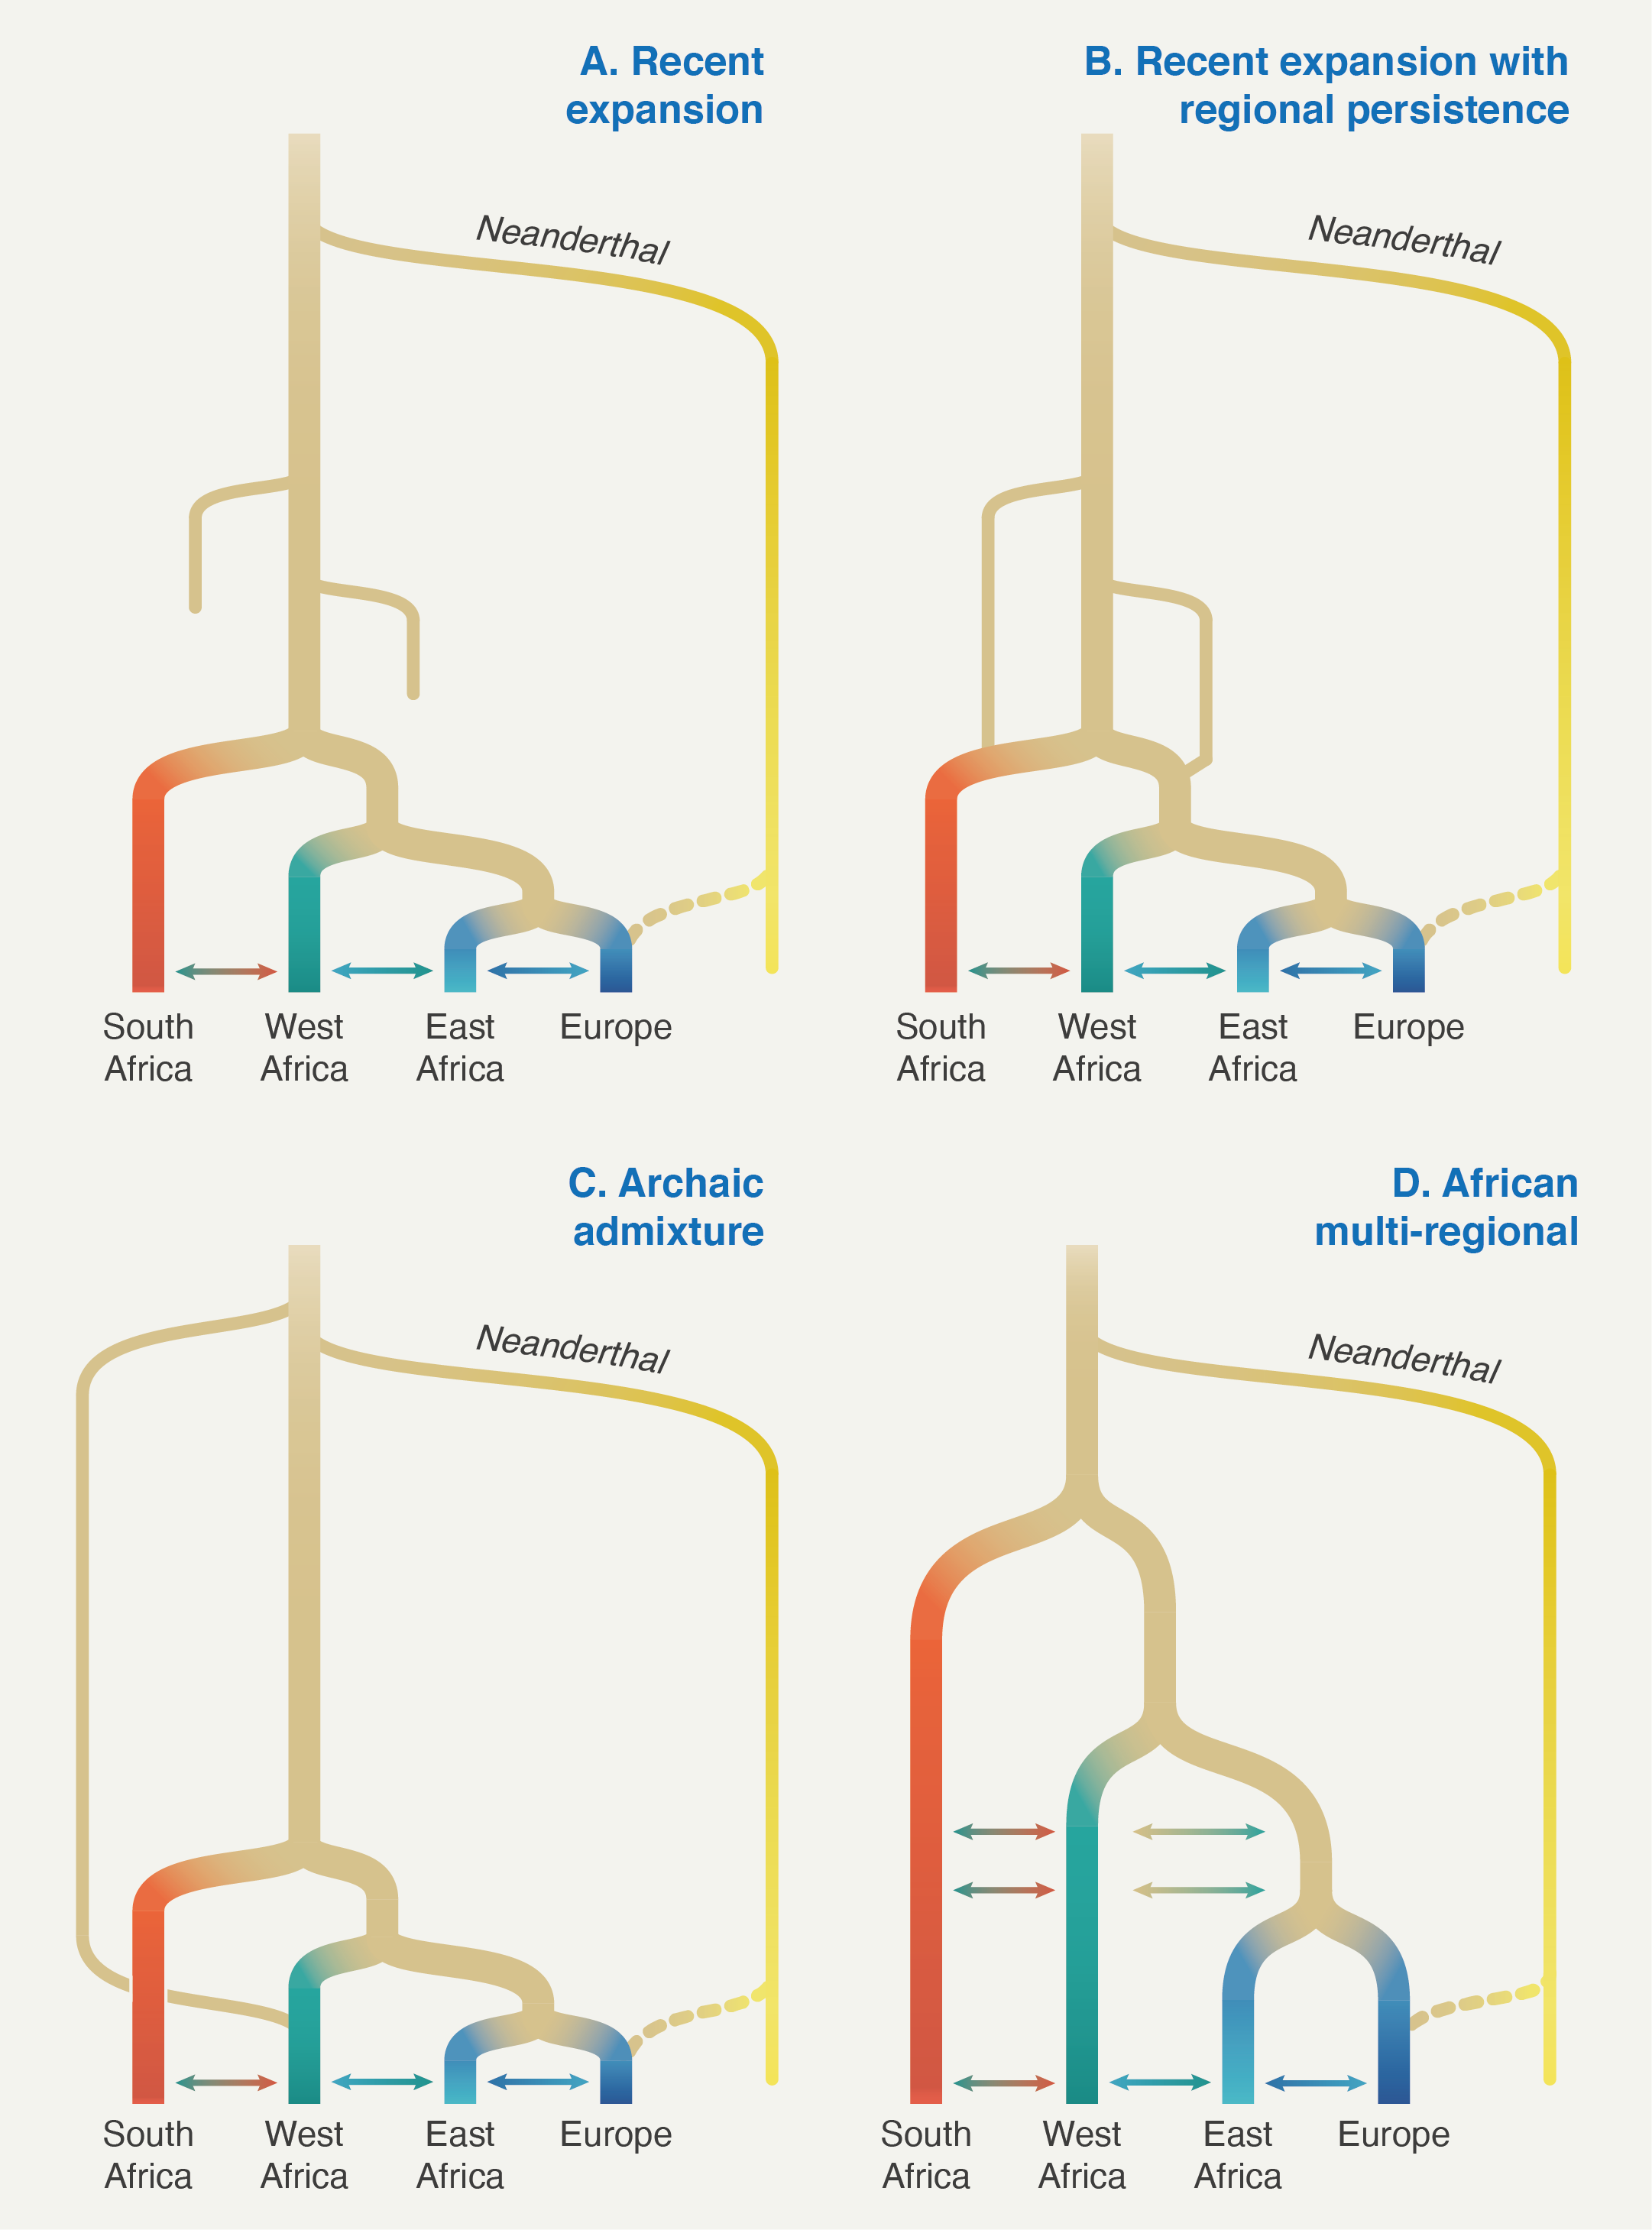
\includegraphics[width=0.65\textwidth]{figures/supp-possible-models.png}
    \caption{\textbf{supp}.}
    \label{fig:supp-possible-models}
\end{center}
\end{figure}


\end{document}
